\section{Architektur der Anwendung}\label{sec:architektur}

Die im letzte Kapitel vorgestellten, theoretischen Konzepte sollen nun in die Praxis umgesetzt werden.
Dazu erläutert dieses Kapitel die Architektur der Anwendung sowie ihre Funktionsweise.
Die Anwendung besteht aus vier Hauptkomponenten: der Klasse \textit{EGraph} mit ihren Hilfsklassen, dem \textit{EGraphService}, dem Server (\textit{server.py}) und der
Weboberfläche (\textit{index.html}). Abbildung~\ref{fig:architektur} gibt einen Überblick über den Zusammenhang zwischen den Komponenten. 

\subsection{Grundlegende Komponenten}

Die erste Komponente bildet die Klasse \textit{EGraph}. Instanzen dieser Klasse implementieren die Datenstruktur E-Graph. Dazu sind fünf weitere Klassen nötig: 
\textit{AbstractSyntaxTreeNode}, \textit{AbstractSyntaxTree}, \textit{RewriteRule}, \textit{ENode} und \textit{EClass}.
Die Klasse \textit{AbstractSyntaxTree} stellt einen AST (\textbf{Abstract Syntax Tree}) dar und benötigt dafür eine Klasse, die die Knoten repräsentiert (\textit{AbstractSyntaxTreeNode}).
Ein mathematischer Ausdruck, aus dem ein E-Graph entstehen soll, wird zuerst in einen AST umgewandelt, was später die Erstellung des E-Graphs vereinfacht.
Die Klasse \textit{RewriteRule} verkörpert eine \textit{rewrite rule}, die aus einem linken und rechten Ausdruck besteht. Beide Ausdrücke werden in einen AST umgewandelt, um das
Anwenden der Regel auf den E-Graph zu vereinfachen.
Die beiden Klassen \textit{ENode} und \textit{EClass} fungieren als Datencontainer, auf die der E-Graph aufbaut.

Die zweite Komponente stellt die Klasse \textit{EGraphService} dar. Über sie läuft die Interaktion zwischen dem Server und einer EGraph-Instanz.
Außerdem regelt sie die Sicherheitsüberprüfungen der Eingabe, z.B. ob ein empfangener Ausdruck vom Server die entsprechende Form aufweist.
Neben diesen Aufgaben ist der Service auch für das Debugging-Feature zuständig. Dieses Feature erlaubt es dem Benutzer, einen E-Graph während verschiedener Operationen
zu beobachten und Informationen über die Vorgehensweise zu erhalten. 

\begin{figure}[H]
  \centering
  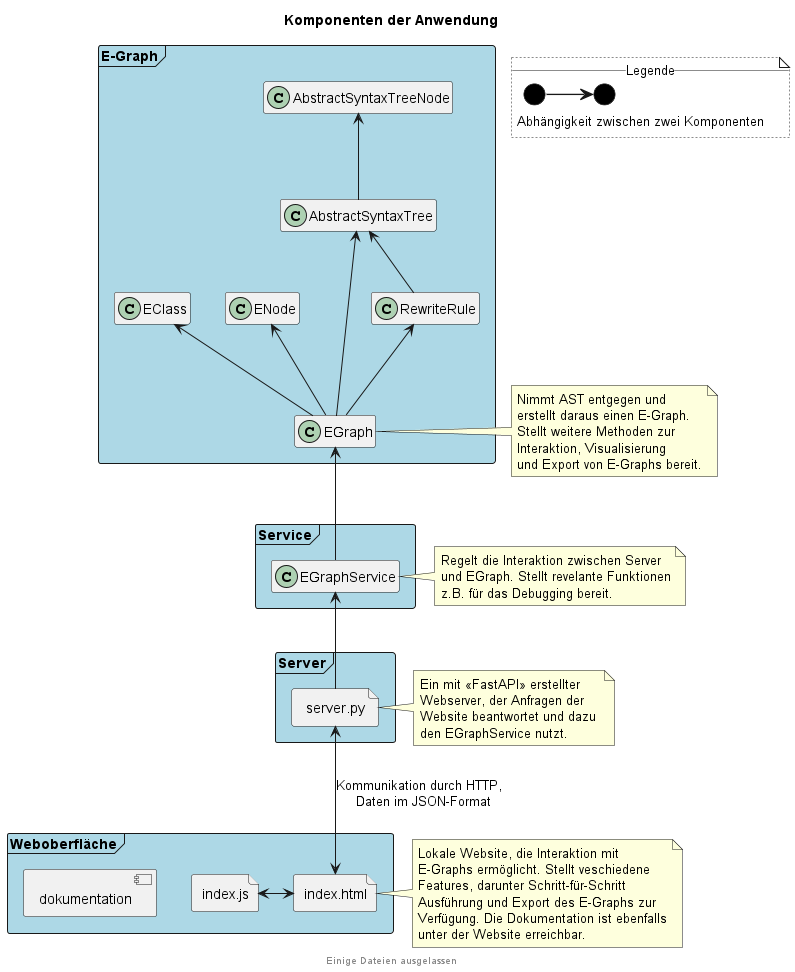
\includegraphics[scale=0.6]{../fig/components.png}
  \caption{Architekturdiagramm der Anwendung}
  \label{fig:architektur}
\end{figure}

Die dritte Komponente ist der Server (\textit{server.py}). Er bildet die Verbindung zwischen dem Service und der Weboberfläche. Für die Umsetzung wurde auf das Framework 
\textit{FastAPI} gesetzt (siehe Kapitel~\ref{sec:entscheidungenundprobleme}). 

Die vierte Komponente bildet die Weboberfläche (\textit{index.html}). Sie läuft lokal im Browser und dient zur Steuerung der Anwendung. Mittels JavaScript können Anfragen an den
Server abgeschickt und Antworten verarbeitet werden.

\subsection{Kommunikation zwischen Server und Weboberfläche}

Zwischen dem Server und der Weboberfläche müssen Daten ausgetauscht werden. Dazu kommunizieren sie das HTTP-Protokoll, während die Daten im 
JSON-Format übertragen werden. Abbildung~\ref{fig:ablauf} zeigt eine beispielhafte Interaktion zwischen Server, Weboberfläche und Benutzer.

Im Beispiel wird die Erstellung eines E-Graphs durch den Benutzer gezeigt. Hierzu gibt der Benutzer einen Ausdruck ein und klickt auf den entsprechenden Button (Abb., Schritt 1).
Das triggert die in JavaScript geschriebene Funktion \textit{create()}. Die Funktion überprüft zuerst, ob es bereits einen E-Graph gibt (Abb., Schritt 2-3) und fragt, ob der Benutzer
diesen und die mit ihm verbundenen Daten löschen will (im Beispiel nicht gezeigt). Falls noch kein E-Graph vorhanden ist, wird nun die Funktion \textit{createEGraph()}
aufgerufen. Sie schickt den Ausdruck an den Server (Abb., Schritt 4) und dieser kümmert sich um die Erstellung. Die Antwort des Servers (Abb., Schritt 5) gibt dem Benutzer 
Auskunft (Abb., Schritt 6), ob dieser Schritt erfolgreich war. 
Anschließend muss der E-Graph und zugehörige \textit{rewrite rules} geladen werden, was durch die Funktion \textit{loadData()} passiert.
Sie schickt eine Anfrage (Abb., Schritt 7), deren Antwort einen Status und die Daten enthält (Abb., Schritt 8). In den Daten befindet sich der entsprechende E-Graph im 
DOT-Format (siehe Kapitel~\ref{sec:entscheidungenundprobleme}), der sogleich als SVG gerendert und auf der Weboberfläche angezeigt wird (Abb., Schritt 9).
In der nächsten Anfrage werden die Regeln geladen (Abb., Schritt 10-11) und anschließend auf der Weboberfläche dargestellt (Abb., Schritt 12).

\begin{figure}[H]
  \centering
  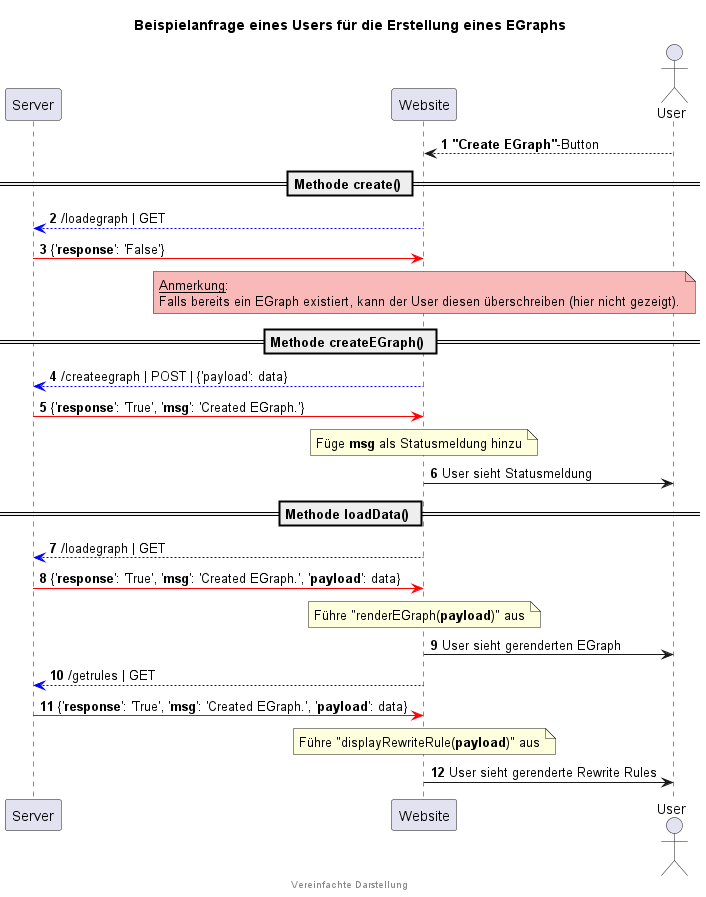
\includegraphics[scale=0.6]{../fig/query.png}
  \caption{Beispielablauf der Kommunikation zwischen Server, Weboberfläche und Benutzer}
  \label{fig:ablauf}
\end{figure}
